\documentclass[11pt,a4paper]{article}
\usepackage[spanish,es-nodecimaldot]{babel}	% Utilizar español
\usepackage[utf8]{inputenc}					% Caracteres UTF-8
\usepackage{graphicx}						% Imagenes
\usepackage[hidelinks]{hyperref}			% Poner enlaces sin marcarlos en rojo
\usepackage{fancyhdr}						% Modificar encabezados y pies de pagina
\usepackage{float}							% Insertar figuras
\usepackage[textwidth=390pt]{geometry}		% Anchura de la pagina
\usepackage[nottoc]{tocbibind}				% Referencias (no incluir num pagina indice en Indice)
\usepackage{enumitem}						% Permitir enumerate con distintos simbolos
\usepackage[T1]{fontenc}					% Usar textsc en sections
\usepackage{amsmath}						% Símbolos matemáticos
\usepackage{listings}
\usepackage{color}

 
\definecolor{codegreen}{rgb}{0,0.6,0}
\definecolor{codegray}{rgb}{0.5,0.5,0.5}
\definecolor{codepurple}{rgb}{0.58,0,0.82}
\definecolor{backcolour}{rgb}{0.99,0.99,0.99}
 
\lstdefinestyle{mystyle}{
    backgroundcolor=\color{backcolour},   
    commentstyle=\color{codegreen},
    keywordstyle=\color{magenta},
    numberstyle=\tiny\color{codegray},
    stringstyle=\color{codepurple},
    basicstyle=\footnotesize,
    breakatwhitespace=false,         
    breaklines=true,                 
    captionpos=b,                    
    keepspaces=true,                 
    numbers=left,                    
    numbersep=5pt,                  
    showspaces=false,                
    showstringspaces=false,
    showtabs=false,                  
    tabsize=2
}
 
\lstset{style=mystyle, language=Python}

% Comando para poner el nombre de la asignatura
\newcommand{\asignatura}{Visión por Computador}
\newcommand{\autor}{José María Sánchez Guerrero}
\newcommand{\titulo}{Cuestionario 1}
\newcommand{\subtitulo}{Filtrado y Detección de regiones}

% Configuracion de encabezados y pies de pagina
\pagestyle{fancy}
\lhead{\autor{}}
\rhead{\asignatura{}}
\lfoot{Grado en Ingeniería Informática}
\cfoot{}
\rfoot{\thepage}
\renewcommand{\headrulewidth}{0.4pt}		% Linea cabeza de pagina
\renewcommand{\footrulewidth}{0.4pt}		% Linea pie de pagina

\begin{document}
\pagenumbering{gobble}

% Pagina de titulo
\begin{titlepage}

\begin{minipage}{\textwidth}

\centering

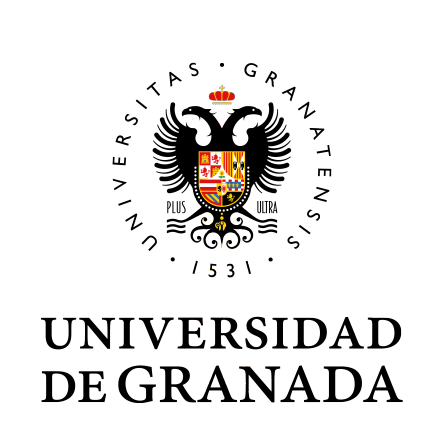
\includegraphics[scale=0.5]{img/ugr.png}\\

\textsc{\Large \asignatura{}\\[0.2cm]}
\textsc{GRADO EN INGENIERÍA INFORMÁTICA}\\[1cm]

\noindent\rule[-1ex]{\textwidth}{1pt}\\[1.5ex]
\textsc{{\Huge \titulo\\[0.5ex]}}
\textsc{{\Large \subtitulo\\}}
\noindent\rule[-1ex]{\textwidth}{2pt}\\[3.5ex]

\end{minipage}

\vspace{0.5cm}

\begin{minipage}{\textwidth}

\centering

\textbf{Autor}\\ {\autor{}}\\[2.5ex]
\textbf{Rama}\\ {Computación y Sistemas Inteligentes}\\[2.5ex]
\vspace{0.3cm}


\includegraphics[scale=0.3]{img/etsiit.jpeg}

\vspace{0.7cm}
\textsc{Escuela Técnica Superior de Ingenierías Informática y de Telecomunicación}\\
\vspace{1cm}
\textsc{Curso 2019-2020}
\end{minipage}
\end{titlepage}

\pagenumbering{arabic}
\tableofcontents
\thispagestyle{empty}				% No usar estilo en la pagina de indice

\newpage

\setlength{\parskip}{1em}


\section*{Ejercicio 1}
\addcontentsline{toc}{section}{Ejercicio 1}

\textbf{Diga en una sola frase cuál cree que es el objetivo principal de la Visión por Computador. Diga también cuál
es la principal propiedad de las imágenes de cara a la creación algoritmos que la procesen.}

El objetivo principal de la Visión por Computador es obtener información significativa de imágenes digitales, posteriormente
analizarla, tratarla y comprender su contenido para tomar decisiones sobre ella de la forma más similar posible a la humana.

Pese a la respresentación en forma matricial de las imágenes que facilita los cálculos a los algoritmos, no podemos centrarnos
únicamente en una posición (píxel) de ésta, ya que los valores alrededor suyo también contienen información relevante sobre él.


\section*{Ejercicio 2}
\addcontentsline{toc}{section}{Ejercicio 2}

\textbf{Expresar las diferencias y semejanzas entre las operaciones de correlación y convolución. Dar una interpretación
de cada una de ellas que en el contexto de uso en visión por computador.}

Ambas son operaciones que transforman localmente una imagen calculado nuevos valores para cada uno de los píxeles. Esto lo hacen
utilizando una máscara 2D de tamaño $NxN$, siendo $N$ un número impar, y aplicándola de la siguiente forma:

Para la correlación:
\begin{equation}
G[i,j]= \sum_{u=-k}^{k} \sum_{v=-k}^{k} H[u,v]F[i+u,j+v]
\end{equation}

Para la convolución:
\begin{equation}
G[i,j]= \sum_{u=-k}^{k} \sum_{v=-k}^{k} H[u,v]F[i-u,j-v]
\end{equation}

Como podemos ver, correlación y convolución son prácticamente iguales, excepto que en la convolución volteamos el filtro antes de
correlacionar. Por ejemplo, convolucionar una imagen 1D con un filtro $(1,3,5)$ sería lo mismo que correlacionarla con el filtro
$(5,3,1)$. En caso de que fuese una convolución 2D voltearíamos tanto horizontal como verticalmente.

Otra cosa que tienen en común es que, como ambos son filtros lineales, ambos cumplen las siguientes propiedades: la \textbf{
superposición}, la cual dice que es lo mismo aplicar una máscara a una composición de imágenes $f_1+f_2$, que aplicarsela a
$f_1$ y a $f_2$ por separado: $h*(f_1 + f_2) = (h*f_1) + (h*f_2)$; y son \textbf{\textit{Shift-Invariant System}}, es decir,
sistemas cuyo valor de entrada no cambian los valores de salida, por lo que no dependen de ellos.

La diferencias más importantes entre ellos es que la convolución es \textbf{conmutativa}, \textbf{distributiva en la adición} y, la
más relevante, \textbf{asociativa}. Es decir, siendo $f$ y $g$ dos filtros distintos, entonces $(f * g)*h = f*(g * h)$. Esto es muy
útil por ejemplo para calcular el filtro \textit{Difference of Gaussian (DoG)}, en el que no tendríamos que convolucionar la imagen
con un filtro Gaussiano y posteriormente con uno derivado, simplemente convolucionaríamos el filtro Gaussiano con el derivado y ya se
lo aplicamos a la imagen.


\section*{Ejercicio 3}
\addcontentsline{toc}{section}{Ejercicio 3}

\textbf{¿Cuál es la diferencia “esencial” entre el filtro de convolución y el de mediana? Justificar la respuesta.}

La principal diferencia entre estos filtros es que el filtro de convolución, como hemos visto antes, es lineal, mientras que el
filtro de mediana no lo es. Para justificar la respuesta veamos un ejemplo: si tenemos los filtros $A=(0,1,2,3,4)$, $B=(5,0,1,4,5)$
y $(A+B)=(5,1,3,7,9)$, el cálculo de sus medianas es:
\begin{equation}
Med(A) = 2 \hspace{10mm} Med(B) = 4
\end{equation}
Y por tanto, como:

\begin{equation}
Med(A)+Med(B)=6 \hspace{5mm} \neq \hspace{5mm} Med(A+B)=5
\end{equation}

podemos justificar que los filtros de mediana no son lineales.

\newpage


\section*{Ejercicio 4}
\addcontentsline{toc}{section}{Ejercicio 4}

\textbf{Identifique el “mecanismo concreto” que usa un filtro de máscara para transformar una imagen.}

El mecanismo que utilizan todos los filtros de máscara para transformar una imagen es que lo hace utilizando \textbf{información local},
es decir, que el valor de cada píxel se calcula teniendo en cuenta los píxeles cercanos a él (los que están dentro de la máscara).

Podremos encontrar varios tipos de filtros, ya sean lineales o no lineales como hemos visto antes, pero ninguno realizará cálculos
en la imagen sin tener en cuenta sus píxeles asociados en la máscara.

\section*{Ejercicio 5}
\addcontentsline{toc}{section}{Ejercicio 5}

\textbf{¿De qué depende que una máscara de convolución pueda ser implementada por convoluciones 1D? Justificar la respuesta.}

Depende de que la máscara de convolución solo se pueda descomponer como producto de dos matrices de dimensión 1. Por ejemplo,
la siguiente máscara Gaussiana se puede descomponer en:

\begin{equation}
\begin{bmatrix}
1 & 2 & 1\\ 
2 & 4 & 2\\ 
1 & 2 & 1
\end{bmatrix}
=
\begin{bmatrix}
1\\
2\\
1
\end{bmatrix}
\begin{bmatrix}
1 & 2 & 1
\end{bmatrix}
\end{equation}


Para comprobar si esto es posible, podemos realizar la \textbf{descomposición en valores singulares} de la matriz. Si esta
descomposición nos da un valor distinto de 0, la máscara será separable en dos matrices 1D, y por tanto, la podremos represetar
como:
\begin{equation}
\sum_{r}^{i=0}\sigma_i u_i v_i^T
\end{equation}
siendo $\sigma_i$ los valores de la matriz diagonal, y $u_i$ y $v_i$ los valores de las respectivas matrices 1D resultantes.

Otra forma que tenemos de comprobarlo es que, si nos fijamos en este tipo de máscaras, el \textbf{rango} de la matriz siempre va
a ser igual a 1.


\section*{Ejercicio 6}
\addcontentsline{toc}{section}{Ejercicio 6}

\textbf{Identificar las diferencias y consecuencias desde el punto de vista teórico y de la implementación entre:}
\begin{enumerate}[label=(\alph*)]
	\item \textbf{Primero alisar la imagen y después calcular las derivadas sobre la imagen alisada}
	\item \textbf{Primero calcular las imágenes derivadas y después alisar dichas imágenes.}
\end{enumerate}
\textbf{Justificar los argumentos.}

Desde un punto de vista teórico dependerá del tipo de filtro que usemos, pero lo lógico sería elegir un filtro de convolución.
Como hemos visto en el ejercicio 2, este filtro tiene cumple la propiedad \textbf{asociativa}, por lo que tanto la opción $a$ como
la $b$ darían el mismo resultado.

\begin{equation}
(f*g)*h=f*(g*h)
\end{equation}

En cuanto a la implementación, es más conveniente \textbf{alisar primero la imagen y posteriormente calcular las derivadas} sobre
la imagen alisada. Si lo hacemos de esta forma, tendremos que hacer solo una convolución y dos derivadas después. De la otra forma,
haremos dos derivadas al principio y posteriormente dos alisamientos, uno para la X y otro para la Y.


\section*{Ejercicio 7}
\addcontentsline{toc}{section}{Ejercicio 7}

\textbf{Identifique las funciones de las que podemos extraer pesos correctos para implementar de forma eficiente la primera derivada de
una imagen. Suponer alisamiento Gaussiano.}




\section*{Ejercicio 8}
\addcontentsline{toc}{section}{Ejercicio 8}

\textbf{Identifique las funciones de las que podemos extraer pesos correctos para implementar de forma eficiente la Laplaciana de una imagen.
Suponer alisamiento Gaussiano.}


\section*{Ejercicio 9}
\addcontentsline{toc}{section}{Ejercicio 9}

\textbf{Suponga que le piden implementar de forma eficiente un algoritmo para el cálculo de la derivada de primer orden sobre una imagen
usando alisamiento Gaussiano. Enumere y explique los pasos necesarios para llevarlo a cabo.}

Los pasos necesarios serían:
\begin{enumerate}
	\item Seleccionar un tamaño para la máscara o calcularlo en función del $sigma$. Podemos poner por ejemplo $6\sigma+1$, ya que con la
	densidad de la función Gaussiana que nos ofrece abarcamos casi toda la máscara.
	\item Calcular los filtros de la primera derivada de la función Gaussiana. Para ello tendremos que muestrear en tantos puntos como
	tamaño hayamos seleccionado anteriormente. También tendremos en cuenta que obtendremos un array para las filas y otro para las columnas.
	\item Normalizar el filtro multiplicando por sigma y hacer la convolución, tanto por filas como por columnas, sobre la imagen.
\end{enumerate}


\section*{Ejercicio 10}
\addcontentsline{toc}{section}{Ejercicio 10}

\textbf{Identifique semejanzas y diferencias entre la pirámide gaussiana y el espacio de escalas de una imagen, ¿cuándo usar una u
otra? Justificar los argumentos.}

Ambas son una representación a distintas escalas de una imagen en las que se utiliza como filtro de suavizado principal el Gaussiano.
También coinciden en la forma de hacer el submuestreo, ya que ambas obtienen la octava de la imagen original, y a partir de ahí siguen
bajando niveles con la imagen resultante.

Se diferencian en que la pirámide Gaussiana únicamente reduce la imagen y obtiene las frecuencias bajas de ella; mientras que en un
espacio de escalas, también se hace uso de estas frecuencias bajas, pero lo hace junto a una serie de técnicas (como puede ser el filtro
Laplaciano sobre el alisamiento o supresión de no másximos) ya que el objetivo de este es detectar las distintas regiones más relevantes
de la imagen. Otra diferencia es que, pese a que se trabaja con una octava de la imagen en cada nivel, esa octava es diferente en una
técnica y otra, porque en el espacio de escalas se realiza cada una de las técnicas comentadas para cada nivel.


\section*{Ejercicio 11}
\addcontentsline{toc}{section}{Ejercicio 11}

\textbf{¿Bajo qué condiciones podemos garantizar una perfecta reconstrucción de una imagen a partir de su pirámide Laplaciana? Dar
argumentos y discutir las opciones que considere necesario.}

Únicamente con las frecuencias altas de la pirámide Laplaciana no podríamos reconstruir la imagen original, también necesitaríamos la 
última submuestra de la imagen, es decir, las frecuencias bajas residuales.

Si disponemos de ella, se podría reconstruir con el siguiente algoritmo, el cual consiste en sumar al último nivel de la Laplaciana
esta última submuestra de frecuencias bajas, y ampliada con una función F:
\begin{equation}
G_k=L_k+F(G_{k+1})
\end{equation}

Cuando terminemos (llegemos a $G_1$) será cuando tengamos la imagen original completamente reconstruida.

\section*{Ejercicio 12}
\addcontentsline{toc}{section}{Ejercicio 12}

\textbf{¿Cuáles son las contribuciones más relevantes del algoritmo de Canny al cálculo de los contornos sobre una imagen? ¿Existe
alguna conexión entre las máscaras de Sobel y el algoritmo de Canny? Justificar la respuesta}

Las contribuciones que tiene este algoritmo frente a otros es que este utiliza las siguientes técnicas:
\begin{enumerate}
	\item \textbf{Non-maximum supression.} Esta técnica recorre todos los píxeles de cada imagen y, para cada uno de ellos, comprueba
	que sus píxeles fronterizos no tienen un valor más alto que el central. En caso de que exista, lo pondrá a cero. Para tener más
	claro cómo funciona, vamos a ejemplificarlo con una matriz ejemplo que represente los píxeles de una imagen:
	\begin{equation*}
		\begin{bmatrix}
		3& 2& 3\\ 
		6& 4& 1\\ 
		1& 3& 3
		\end{bmatrix}
		\underset{(x,y)>=(0,0)}{\rightarrow}
		\begin{bmatrix}
		3& 2& 3\\ 
		6& 0& 1\\ 
		1& 3& 3
		\end{bmatrix}
		\hspace{10mm}
		\begin{bmatrix}
		3& 2& 3\\ 
		1& 4& 1\\ 
		1& 3& 3
		\end{bmatrix}
		\underset{(x,y)<(0,0)}{\rightarrow}
		\begin{bmatrix}
		0& 0& 0\\ 
		0& 4& 0\\ 
		0& 0& 0
		\end{bmatrix}
	\end{equation*}
	A la izquierda vemos que hay valores mayores que el central, el $(1,0)=6$, asi que el píxel central termina siendo cero. Por otra parte, en
	la matriz de la izquierda, ningun valor es más grande que el central, por lo que podemos decir que es un máximo.

	\item \textbf{Linking and thresholding (hysteresis).} Tras hacer la supresión de no máximos, define dos umbrales (thresholding), uno alto
	y otro bajo. Volveremos a recorrer cada píxel y dependiendo su valor con los umbrales se hará lo siguiente: en caso de ser inferior que el
	bajo, no se le considerará como borde; si está entre bajo y el alto, será parte del borde si está conectado a otro que ya está considerado
	como borde; y si el valor es superior al umbral alto, se le considerará como borde.

	Antes de aplicar estas dos técnicas, Canny tiene que encontrar la magnitud y orientación del gradiente. Para ello se servirá de las
	\textbf{máscaras de Sobel}, las cuales se basan en el cálculo de la primera derivada respecto de X e Y.

\end{enumerate}


\section*{Ejercicio 13}
\addcontentsline{toc}{section}{Ejercicio 13}

\textbf{Identificar pros y contras de k-medias como mecanismo para crear un vocabulario visual a partir del cual poder caracterizar patrones.
¿Qué ganamos y que perdemos? Justificar los argumentos}

K-means es un algoritmo de clasificación no supervisado el cual selecciona un número de clústeres y sus centros. Después, clasifica cada punto
de los descriptores calculando la distancia entre ellos y el centro más cercano, minimizando el error de la suma de cuadrados; y por último
recalcula los centros de cada cluster.

Es de los algoritmos más utilizados y más populares, ya que entre sus principales \textbf{ventajas} tenemos:
\begin{itemize}
	\item Simplicidad y velocidad que le permite ejecutarse en grandes conjuntos de datos. Su complejidad computacional por cada iteración es
	de: asignar cada punto al centro del cluster más cercano $O(n*k)$, y recalcular el centro del cluster a la media de sus puntos asignados $O(n)$.
	\item Utiliza "hard assignment", es decir, cada punto se asigna a únicamente un solo cluster.
	\item Su simplicidad facilita la demostración de los resultados obtenidos, a diferencia de las redes neuronales o las SVM.
	\item Que sea eficiente implica que el algoritmo es bueno por si necesitamos segmentar el conjunto de datos.
\end{itemize}

Entre sus \textbf{desventajas} tenemos que:
\begin{itemize}
	\item Los centros de los k clusters iniciales se inicializan aleatoriamente, asi que no se produce el mismo resultado tras cada ejecución.
	Una mala inicialización	nos puede llevar a: una mala velocidad de convergencia y a un mal agrupamiento de los clusteres.
	\item Necesita el número de clústeres que se especificarán. Demasiados clústeres pueden causar escasez de datos y muy pocos pueden provocar que
	llegen a converger, por eso hay que elegir con cuidado.
	\item No garantiza que el resultado sea un mínimo global de la varianza, ya que converge a un óptimo local.
	\item Sensible a los valores atípicos. Cuando hay valores atípicos, los centros de los clusteres resultantes pueden no ser tan representativos y,
	por lo tanto, el error de la suma de cuadrados (varianza) también será más alto, y nuestro objetivo en minimizarlo.
	\item No trabaja bien con grupos no lineales.
\end{itemize}


\section*{Ejercicio 14}
\addcontentsline{toc}{section}{Ejercicio 14}

\textbf{Identifique pros y contras del modelo de “Bolsa de Palabras” como mecanismo para caracterizar el contenido de una imagen. ¿Qué ganamos y
que perdemos? Justificar los argumentos.}

El modelo de 'Bolsa de Palabras' extrae las características locales de una imagen, muestrea un subconjunto de ellas y construye un diccionario
visual mediante \textit{k-means} visto en el ejercicio anterior, cuantifica las característica utilizando este diccionario, y por último, representa
imágenes mediante la frecuencia de cada 'palabra visual'. Veamos las \textbf{ventajas} de usar este método:
\begin{itemize}
	\item Es bastante flexible a la geometría o las deformaciones producidas por el punto de vista (donde hayamos tomado la imagen).
	\item Resume bastante bien el contenido de la imagen.
	\item Proporciona una representación vectorial para imágenes y poder crear así un histograma.
	\item En la práctica, nos ofrece buenos resultados.
\end{itemize}

Como \textbf{desventajas} tenemos que:
\begin{itemize}
	\item Generar el vocabulario a partir de grandes cantidades de datos suele ser computacionalmente costoso.
	\item El modelo básico no tiene en cuenta la geometría, asi que tendrá que verificar después o codificar mediante funciones.
	\item Para los humanos, intuitivamente vemos la división de los objetos en partes, pero realmente esa información no existe. Por tanto, no
	tenemos	grantías de capturar todos los puntos de interés.
	\item Si la bolsa de palabras cubre toda la imagen, se puede mezclar el fondo y el primer plano. Para solucionarlo se suelen utilizar las
	pirámides espaciales.
	\item Sigue siendo complicado la formación del vocabulario óptimo, al igual que todavía no ha sido ampliamente testeado para invarianza
	en la escala y en el punto de vista.
\end{itemize}


\section*{Ejercicio 15}
\addcontentsline{toc}{section}{Ejercicio 15}

\textbf{Suponga que dispone de un conjunto de imágenes de dos tipos de clases bien diferenciadas. Suponga que conoce como implementar de forma
eficiente el cálculo de las derivadas hasta el orden N de la imagen. Describa como crear un algoritmo que permita diferenciar, con garantías,
imágenes de ambas clases. Justificar cada uno de los pasos que proponga.}

Como sabemos calcular de manera eficiente las derivadas hasta el orden N, yo utilizaría un espacio de escalas y así obtener las características
invariantes a la escala. Después haríamos la supresión de no máximos, pero eliminando los contornos porque si no, nos encontraríamos ahí a la
mayoría de máximos. A continuación, realizamos el cálculo del gradiente para cada punto obtenido y se crea el histograma con las mayores
frecuencias de direcciones. Por último, ya podemos pasar a extraer las características con un algoritmo.

Este algoritmo consistirá en una 'Bolsa de palabras', en el cual aprenderemos un 'vocabulario visual' muestreando un subconjunto de características
y después utilizando un algoritmo de clustering como el \textit{k-means}. Cuantificamos las características utilizando este diccionario y para terminar
ya sólo nos faltaría un clasificador, y como las características deben de estar bien diferenciadas si hemos hecho correctamente los pasos anteriores,
yo utilizaría un SVM o kNN para separarlas.

\end{document}